%!TEX root = ../thesis.tex
%*******************************************************************************
%*********************************** Analysis Overview *********
%*******************************************************************************

\chapter{Analysis overview}\label{ch:1lepton}

\ifpdf
    \graphicspath{{chapter-analysis/Figs/Raster/}{chapter-analysis/Figs/PDF/}{chapter-analysis/Figs/}}
\else
    \graphicspath{{chapter-analysis/Figs/Vector/}{chapter-analysis/Figs/}}
\fi


This chapter aims to give an introduction to the search for electroweakinos presented in this work. First, the targeted final state, the 1-lepton final state, is introduced and motivated, followed by the \gls{sm} background processes that need to be considered when doing searches for \gls{susy} in this final state. Next the reconstruction and identification of physics objects as well as the event selection requirements are described.

\section{Search for electroweakinos in the 1-lepton final state}


\textsc{MadGraph5\_aMC@NLO} 2.6.2~\cite{MGaMCNLO:2014hca,Frederix:2012ps}


\section{Standard Model backgrounds}

\begin{figure}
	\centering
	\begin{subfigure}[b]{0.3\linewidth}
		\centering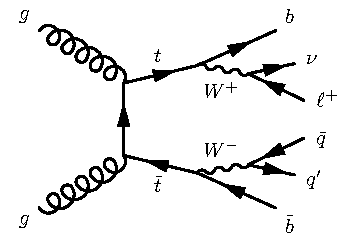
\includegraphics[width=\textwidth]{ttbar}
		\caption{\label{fig:ttbar}}
	\end{subfigure}\quad
	\begin{subfigure}[b]{0.3\linewidth}
		\centering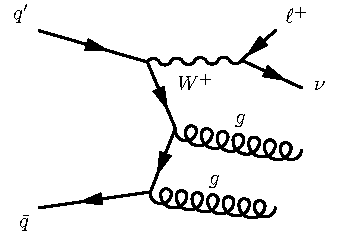
\includegraphics[width=\textwidth]{wjets}
		\caption{\label{fig:wjets}}
	\end{subfigure}\quad
%	\begin{subfigure}[b]{0.25\linewidth}
%		\centering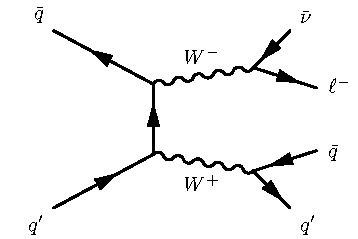
\includegraphics[width=\textwidth]{diboson}
%		\caption{\label{fig:diboson}}
%	\end{subfigure}
	\begin{subfigure}[b]{0.3\linewidth}
		\centering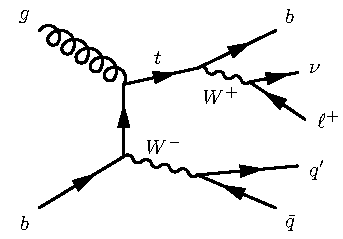
\includegraphics[width=\textwidth]{singletop}
		\caption{\label{fig:singletop}}
	\end{subfigure}	
	\caption{Exemplary Feynman diagrams showing the dominant processes \subref{fig:ttbar} $t\bar{t}$, \subref{fig:wjets} $W+\textrm{jets}$ and \subref{fig:singletop} single top production with subsequent decays.}
	\label{fig:sm_backgrounds_feynman}
\end{figure}

Although the requirement of exactly one lepton isolated from surrounding hadronic activity significantly reduces the contribution from \gls{qcd} multi-jet background, numerous \gls{sm} processes can result in final states with exactly one isolated lepton, multiple jets and missing transverse momentum. Background sources are generally classified into \textit{reducible} and \textit{irreducible} backgrounds. Irreducible backgrounds are processes that have a physical phase space that is indistinguishable from the final state of the signal process considered. Reducible backgrounds, on the other hand, result from partially misreconstructed processes as well as mismeasurements. Examples of reducible processes are events where a lepton originates from a \gls{hf} decay, photon conversions or misreconstructed jets. \gls{sm} processes that result in final states with an isolated lepton, multiple jets and missing transverse momentum typically involve a $W$ boson decaying into a lepton--neutrino pair (a so-called \textit{leptonic decay}). The neutrino will contribute to the total missing transverse momentum in the event, while additional jets can appear in the final state through \gls{qcd} radiation or other branches of the decay chain.

By far the largest \gls{sm} background contributions stem from the production of top quarks, including top quark pair $\ttbar$ production as well as single top processes. These processes were generated using \textsc{Powheg-Box} v2~\cite{PowhegBox:2010xd}, implementing the \textsc{POWHEG} method~\cite{Powheg1,Powheg2} for merging \gls{nlo} \glspl{me} with the \glspl{ps}. The \gls{ps}, hadronisation and underlying event were simulated using \textsc{Pythia8.230}~\cite{Pythia8:2007gs} with the A14 set of tuned parameters~\cite{ATL-PHYS-PUB-2014-021}. Contributions from $\ttbar$ production in association with a vector boson $\ttbar+V$ (\textit{W} or \textit{Z}) are relatively small, but still considered in the background estimation. It is simulated using \textsc{MadGraph5\_aMC@NLO} 2.3.3 and \textsc{Pythia8} using the A14 tune. The set of \glspl{PDF} used for simulation of $\ttbar$, single top, and $\ttbar+V$ is the NNPDF 2.3 LO~\cite{Ball:2012cx} set.

Apart from processes involving top quarks, the production of the vector bosons \textit{W} and \textit{Z} constitutes another major source of \gls{sm} backgrounds. Production of a vector boson $V$ with additional jets ($V+\mathrm{jets}$) is simulated using \textsc{Sherpa} 2.2.1~\cite{Gleisberg:2008ta,Bothmann:2019yzt}, allowing up to two (four) additional parton emissions at NLO (LO) accuracy. The CKKW \gls{me}+\gls{ps} matching and merging scheme~\cite{Hoeche:2009rj,Catani:2001cc}, extended to NLO accuracy~\cite{Hoeche:2012yf}. The \glspl{PDF} used are provided by the NNPDF 3.0 NNLO set~\cite{Ball:2014uwa}. While $W(\rightarrow\ell\nu)+\mathrm{jets}$ is a major background in this analysis, $Z+\mathrm{jets}$ plays only a minor role, as the only irreducible component is $Z(\rightarrow\tau\tau)+\mathrm{jets}$, where one $\tau$-lepton undergoes a leptonic decay and the other one a hadronic decay. Other $Z+\mathrm{jets}$ processes are reducible and typically produce not enough $\etmiss$ to end up in the same phase space as signal processes. Production of of pairs ($VV$) and triplets ($VVV$) of vector bosons, called \textit{diboson} and \textit{multiboson} production, respectively, is simulated using \textsc{Sherpa} 2.2.1 and 2.2.2.

Various \gls{sm} processes involving Higgs bosons can also result in final states with one lepton, two $b$-tagged jets (from $h\rightarrow b\bar{b}$), and $\etmiss$ and, although their contributions are overall relatively small, are thus included in the background estimation. The processes considered in this analysis include Higgs boson production in association with a top-quark pair or a vector boson ($h+\ttbar$ and $h+V$) as well as single Higgs production through \gls{vbf} or \gls{ggf}. All Higgs processes are simulated using \textsc{Powheg-Box} for the \gls{me} calculations and \textsc{Pythia8} for the \gls{ps}, underlying event and hadronisation. 

Pure \gls{qcd} multi-jet events---omnipresent at hadron colliders like the \gls{lhc}---can only appear in the 1-lepton final state through false reconstruction of a jet as a lepton (so-called \textit{fake} leptons) and mismeasurement of $\etmiss$. As it has been shown that this background is negligible in all selections relevant to this search, no estimation for \gls{qcd} contribution is considered in the following~\cite{SUSY-2019-08}.

\Cref{fig:sm_backgrounds_feynman} shows exemplary Feynman diagram for the production and decay of the major backgrounds considered in this analysis, $\ttbar$, single top and $\wjets$. \Cref{tab:mc_generators} summarises all \gls{mc} generators and software versions used for the simulated events used in the following. Further details are given in the relevant ATLAS simulation notes~\cite{ATL-PHYS-PUB-2018-009,ATL-PHYS-PUB-2016-005,ATL-PHYS-PUB-2017-006,ATL-PHYS-PUB-2017-005,ATL-PHYS-PUB-2016-002}.

\section{Monte Carlo samples}

\begin{table}
	\centering
	\setlength\heavyrulewidth{0.2ex}
	\small
	\caption{Overview of configuration of \gls{mc} generators used for simulating the various signal and \gls{sm} background processes.}
	\resizebox{\textwidth}{!}{\begin{tabular} {llllll}
	\toprule
	Process & Matrix element & Parton shower & PDF set & Cross section & Tune\\ 
	\midrule
	Signal & \textsc{MadGraph5\_aMC@NLO} 2.6.2 & \textsc{Pythia} 8.230 & NNPDF 2.3 LO & NLO+NLL ??? & ATLAS A14 \\
	\midrule	
	$\ttbar$ & \textsc{Powheg-Box} & \textsc{Pythia} 8.230 & NNPDF 2.3 LO & NLO+NLL ??? & A14 \\
	$t$ (s-channel) & \textsc{Powheg-Box} & \textsc{Pythia} 8.230 & NNPDF 2.3 LO & NLO+NLL ??? & A14 \\
	$t$ (t-channel) & \textsc{Powheg-Box} & \textsc{Pythia} 8.230 & NNPDF 2.3 LO & NLO+NLL ??? & A14 \\
	$t+W$ & \textsc{Powheg-Box} & \textsc{Pythia} 8.230 & NNPDF 2.3 LO & NLO+NLL ??? & A14 \\
	$\ttbar + V$ & \textsc{MadGraph5\_aMC@NLO} 2.3.3 & \textsc{Pythia} 8.210 & NNPDF 2.3 LO & NLO+NLL ??? & A14 \\
	\midrule
	$V+\mathrm{jets}$ & \multicolumn{2}{c}{\textsc{Sherpa} 2.2.1} & NNPDF 3.0 NNLO & NNLO ??? & \textsc{Sherpa} default \\
	$VV$ & \multicolumn{2}{c}{\textsc{Sherpa} 2.2.1/2.2.2} & NNPDF 3.0 NNLO & NNLO ??? & \textsc{Sherpa} default\\
	$VVV$ & \multicolumn{2}{c}{\textsc{Sherpa} 2.2.1/2.2.2} & NNPDF 3.0 NNLO & NNLO ??? & \textsc{Sherpa} default\\
	\midrule
	$h+\ttbar$ & \textsc{Powheg-Box} & \textsc{Pythia} 8.230 & NNPDF 2.3 LO & NLO+NLL ??? & A14 \\
	$h+V$ & \textsc{Powheg-Box} & \textsc{Pythia} 8.212 & NNPDF 3.0 NNLO & NLO+NLL ??? & AZNLO \\
	\textit{h (ggF)} & \textsc{Powheg-Box} & \textsc{Pythia} 8.212 & NNPDF 3.0 NNLO & NLO+NLL ??? & AZNLO \\
	\textit{h (VBF)} & \textsc{Powheg-Box} & \textsc{Pythia} 8.212 & NNPDF 3.0 NNLO & NLO+NLL ??? & AZNLO \\
	\bottomrule
	\end{tabular}}\vspace{3mm}
	\label{tab:mc_generators}   
\end{table}

\section{Object definitions}

\section{Event selection}

\section{Triggers}